\documentclass[Main.tex]{subfiles}

\begin{document}
\section{Equilibri, stabilità e piccole oscillazioni} \toc


\subsection{Introduzione}
Il sistema in esame è della forma
\begin{equation}
	\L = \frac{1}{2} \dot q \cdot A(q) \dot q - \U (q) = \K_2 - \U
\end{equation}
La prima cosa da ricordare è a legge di conservazione dell'energia, ovvero esiste una costante del moto che è delle forma
\begin{equation}
	H= \K_2 + \U = E
\end{equation}
Le equazioni di Lagrange in forma generale sono
\begin{equation}
	\ddot q = -A^{-1}(q) \left[ \gamma (\dot q) + \pp{\U}{q} \right] \iff \begin{cases}
 	\dot q = v\\
 	\dot v = -A^{-1} (q)\left[ \gamma (\dot q) + \pp{\U}{q} \right] 
 \end{cases}
\end{equation}

\subsection{Equilibri}
\begin{df}[equilibrio]
Si definiscono equilibri del sistemi lagrangiano, gli zeri del campo vettoriale
\begin{equation}
	Y(q,v):=\vec{v \\ -A^{-1} (q)\left[ \gamma (\dot q) + \pp{\U}{q} \right]}
\end{equation}
Cioè $v=0 \Rightarrow \gamma(0)=0$ e $A^{-1} \pp{\U}{q}(q)=0$ e ovvero, moltiplicando per $A$ ambo i membri.
\begin{equation}
	\Rightarrow \pp{\U}{q}(q)=0
\end{equation}
I punti di equilibrio nello spazio delle fasi sono della forma 
\begin{equation}
	\vec{ \overline q \\ 0}\text{ con } \pp{\U}{\overline q}=0
\end{equation}
\end{df}

\subsubsection{Linearizzazione del sistema attorno al punto di equilibrio $(\overline q  \ 0 )$}
Dato $q(t) = \bar q + \xi(t)$ e $v(t) = (0+) \eta (t)$ si può scrivere il sistema
\begin{gather}
	\begin{cases}
		\dot \xi = \eta \\
		\dot \eta = -A^{-1} ( \bar q + \xi ) \left[\gamma(\eta) + \pp{\U}{q} ( \bar q + \xi) \right]
	\end{cases}
\end{gather}
Si sta quindi espandendo per $\xi$ e $\eta$ piccoli attorno a un punto di equilibrio. Lo sviluppo di $A^{-1}$ e $\gamma$ sembra complicato, in realtà $\gamma (\eta)$ è una forma quadratica di $\eta$ quindi è già $o(2)$ e quindi il prodotto $A^{-1} ( \bar q + \xi ) \gamma(\eta)$ è trascurabile per l'ordine 1. Il termine $\pp{\U}{q} ( \bar q + \xi)$ al primo ordine ha un contributo nullo in $\bar q$ per definizione di $\bar q$ + un termine lineare in $\xi$, il prodotto $A^{-1} ( \bar q + \xi )\pp{\U}{q} ( \bar q + \xi)$ allora ha una parte quadratica in $\xi$ e quindi anche questa parte è $o(2)$. L'unica cosa da sviluppare è quindi è $\pp{\U}{q}$. In modo esplicito si ha:
\begin{gather}
	\pp{\U}{q}= -A^{-1} (\bar q) \left[ \cancelto{0}{\pp{\U}{q} (\bar q)} +\pp{^2 \U}{q^2}(\bar q) \xi \right] + \underset{\underset{\text{in $\xi$ e $\eta$}}{\uparrow}}{o(2)}
\end{gather}
Quindi il sistema linearizzato (attorno al punto di equilibrio) è 
\begin{equation}
	\begin{cases}
		\dot \xi = \eta \\
		\dot \eta = -A^{-1}(q) \pp{^2 \U}{q^2}(\bar q) \xi 
	\end{cases}
\end{equation}
In particole $\pp{^2 \U}{q^2}(\bar q)$ è l'hessiano 
\begin{equation}
	\left( \pp{^2 \U}{q^2}(\bar q) \right)_{ij} = \pp{^2 \U }{q_\ell \partial q_m} (\bar q) 
\end{equation}
La matrice hessiana per costruzione è una matrice simmetrica, il segno invece dipende da $\U$ ed è $\neq 0$ se il punto di equilibrio è non degenere; nel caso in cui fosse degenere tutta la matrice sarebbe nulla e quindi bisognerebbe calcolare ordini successivi. 

Rinominando $ \bar A := A(\bar q) $ e $\bar B := \pp{^2 \U}{q^2}(\bar q)$ si può riscrivere
\begin{gather} \label{minimo}
	\begin{cases}
		\dot \xi = \eta \\
		\dot \eta = - \bar A^{-1} \bar B \xi 
	\end{cases} \iff \ddot \xi =- \bar A^{-1} \bar B \xi \iff \boxed{\bar A \ddot \xi = - \bar B \xi }
\end{gather}
Questa equazione vettoriale per $A$ e $B$ positivi è l'equazione di un'oscillatore armonico con frequenza $\nu =\sqrt{\frac{B}{A}}$, invece è un repulsore armonico se $\bar B <0$. $\bar A$ si è già dimostrato essere definita positiva, quindi per un minimo locale non degenere dell'energia potenziale, che corrisponde al caso $\bar B$ definita positiva, la \eqref{minimo} è l'equazione dell'osicillatore armonico. Se $\bar B$ è definita negativa, ovvero si ha un massimo dell'energia potenziale in $\bar q$, allora la \eqref{minimo} è quella di un repulsore armonico. Esistono inoltre situazioni in cui non tutti gli autovalori siano strettamente positivi o negativi e quindi si viola la condizione di punto critico non degenere.


	Per studiare il caso di un minimo non degenere si cercano prima soluzione della forma 
	\begin{equation}
		\xi(t) = u \cos ( \omega t)
	\end{equation}
	Si può mettere anche $\sin(\omega t)$ o una combinazione lineare delle due, in questa equazione $u \in \Rr^L$.
	Se inserita dentro la \eqref{minimo} si ottiene un equazione del tipo
	\begin{equation}
		\ddot \xi (t) = - \omega^2 u \cos ( \omega t) = - \omega^2 \xi 
	\end{equation}
	Allora si riconoscono i termini
	\begin{gather}
		- \omega^2 ( \bar A u) \cancel{\cos( \omega t)} = - ( \bar B u) \cancel{(\cos \omega t )}\\
		\rightarrow \omega^2 \bar A u = \bar B u \iff  (\omega^2 \bar A - \bar B ) u=0
	\end{gather}
	Se $A$ fosse l'identità questa sarebbe  esattamente l'equazione che definisce gli autovalori e gli autovettori di $\bar B$. Quindi è una \emph{complicazione} rispetto al problema  cosiddetto secolare, quello agli autovalori, che coinvolge due matrici invece che una sola. Questo problema è anche detto problema caratteristico per piccoli oscillazioni attorno al minimo.
	
	\begin{osservazioni}
		\item Se si cerca una soluzione generica della forma
		\begin{gather}
			\xi (t) = u c(t)
		\end{gather}
		Una volta inserita nell'equazione si ottiene
		\begin{gather}
			\bar A (\ddot c (t) u ) = \bar B c(t) u
			\iff \ddot c(t) \bar A u = - c (t) \bar B u\\
			\ddot c(t) u \cdot \bar A u = -c(t) u \cdot \bar B u\\
			\longrightarrow \frac{\ddot c(t)}{c(t)} = - \frac{u \cdot \bar B u}{u \cdot \bar A u} \ \ \ (\forall u \cancel \equiv 0, \text{ e } \forall t: c(t) \neq 0)
		\end{gather}
		Questa identità implica che $\frac{\ddot c (t)}{c(t)} = \text{cost} < 0 $ (se $\bar B$ è definita positiva) o in maniera equivalente 
		\begin{gather}
			\frac{\ddot c(t)}{c(t)} = - \omega^2 \Rightarrow -\omega^2 = -\frac{u \cdot \bar B u }{u \cdot \bar A u}\\
			\ddot c = - \omega^2 c \Rightarrow -\omega^2 \cancel{c} \bar A u = - \cancel{c} \bar B u\\
			\Rightarrow \omega^2 \bar A u = \bar B u
		\end{gather}
		Quindi in maniera automatica si che $c(t)$ è una soluzione di tipo armonico.
		\item Se si trovano $L$ corpi con $(\omega_i^2, u_i)$, con gli $u_i$ linearmente indipendenti allora la soluzione generale è 
		\begin{equation}
			\xi(t) = \sum_{i=1}^L c_i (t) u_i
		\end{equation}
		Con $c_i(t) = a_i \cos (\omega_i t) + b_i \sin (\omega_i t )$
		
		\item La trattazione svolta fin'ora è sostanzialmente lo sviluppo della lagrangiana fino all'ordine 2:
		\begin{gather}
			\L = \K_2 - \U = \frac{1}{2} \dot q \cdot A(\bar q) \dot q - \U(q)
		\end{gather}
		Attorno all'equilibrio $\vec{ \bar q \\ 0 }\Rightarrow \begin{cases}
 				q(t) = \bar q + \xi (t) \\
 		 		\dot q = \dot \xi (t)	
 			\end{cases}$
		\begin{gather}
			\Rightarrow \L = \frac{1}{2} \dot \xi \cdot \underbrace{A(\bar q + \xi ) }_{A ( \bar q) +o(1)} \dot \xi - \underbrace{\U (\bar q + \xi)}_{\U(\bar q) + \cancel{\pp{\U}{q} (\bar q)} \xi + \frac{1}{2} \xi \cdot \pp{^2\U}{q^2} (\bar q) \xi + o(3)}\\
			\L_2 + o(3)
		\end{gather}
		Dove $\L_2$ è 
		\begin{equation}
			\L_2 = \frac{1}{2} \dot \xi \cdot \bar A \dot \xi - \frac{1}{2} \xi \cdot \bar B \xi \textcolor{gray}{ - \U(\bar q)}
		\end{equation}
		E poi dalle equazioni di Lagrange si è ottenuto $\bar A \ddot \xi = - \bar B \xi $
	\end{osservazioni}

\newpage
\begin{teo}[di Lagrange] Siano $\bar A$ e $\bar B$ simmetriche e definite positive allora
\begin{enumerate}
	\item L'equazione caratteristica $\omega^2 \bar A u = \bar B u$ ammette $L$ soluzioni $(\omega_i^2, u_i), \ i=1, \dots ,L$ con $u_i, \dots , u_L$ linearmente indipendenti e la soluzione generale di $\bar \ddot \xi = - \bar B \xi $ è data da 
	\begin{equation}
		\xi(t) = \sum_{i=1}^L c_i(t) u_i
	\end{equation} 
	
	\item Nelle coordinate $c_i$ si ha che $\L_2$ è diagonalizzata, o separata, in lagrangiane di oscillatore armonico
	\begin{equation}
		\L_2 = \sum_{i=1}^L \left( \frac{1}{2} \dot c^2_i - \frac{1}{2} \omega_i^2 c_i^2 \right)
	\end{equation} 
\end{enumerate}
\end{teo}

\begin{dm}
\begin{enumerate}
	\item Partendo dall'equazione caratteristica
\begin{gather}
	\omega^2 \bar A u = \bar B u \ \ \ \ \left( \omega^2 = \frac{u \cdot \bar b u}{u \cdot \bar Au} > 0 \ \forall u \cancel \equiv 0 \right)\\
	\iff ( \omega^2 \bar A - \bar B ) u =0 
\end{gather}	
Se il determinante di $\omega^2 \bar A - \bar B $ fosse diverso da 0 allora sarebbe invertibile, si potrebbe moltiplicare per l'inversa a destra e sinistra e si otterebbe $u \equiv 0$ che è una soluzione banale. Allora si richiede che 
\begin{gather}
	\Rightarrow \det ( \omega^2 \bar A - \bar B )=0
\end{gather}
Cioè è l'equazione caratteristica per gli autovalori o per le frequenze caratteristice
\begin{osservazione}
	Siccome è noto che $\bar A$ sia simmetrica, invertibile e positiva si può scrivere
	\begin{gather}
		\text{det} ( \bar A ( \omega^2 \1 - \bar A ^{-1} \bar B ) = \\ = \det \bar A \det (\omega^2 \1 - \bar A^{-1} \bar B ) =0
	\end{gather}
	Quindi $\omega^2$ sono gli autovalori della matrice $\bar A^{-1} \bar B$. Oppure si può scrivere
	\begin{gather*}
		\det ( \bar A \omega^2 - \bar B ) =\\ = \det ( \bar A^{1/2} ( \omega^2 \1 - \bar A^{-1/2} \bar B \bar A^{-1/2} ) \bar A ^{1/2} )=\\
		= (\det \bar A^{1/2} )^2 \det  ( \omega^2 \1 - \bar A^{-1/2} \bar B \bar A^{-1/2} )=0
	\end{gather*}
	Così si sta cercando gli autovalori per una matrice $\bar A^{-1/2} \bar B \bar A^{-1/2} $ simmetrica reale ($A$ e $B$ sono reali) e definita positiva. Per il teorema spettrale i suoi autovalori sono anch'essi reali. Per convincersi della simmetria si fa la trasposta
	\begin{gather}
		( \bar A^{-1/2} \bar B \bar A^{-1/2} )^T =\\= (\bar A^{-1/2})^T( \bar B)^T ( \bar A^{-1/2})^T  = \bar A^{-1/2} \bar B \bar A^{-1/2} 
	\end{gather}
	Per convincersi del segno si fa
	\begin{gather*}
		u \cdot ( \bar A^{-1/2} \bar B \bar A^{-1/2} )u = ( \underbrace{\bar A^{-1/2} u}_{v}) \cdot (B ( \underbrace{\bar A^{-1/2} u}_{v}) = \\
		v \cdot \bar B v \begin{cases}> 0 \ \forall v \neq 0 \\
		=0 \ \ \text{se } v= 0 \iff \bar A^{-1/2}u = 0 \iff u=0 \end{cases}
	\end{gather*}
	Quindi le $\omega_i^2$ sono gli autovalori (positivi) di $\bar A^{-1/2} \bar B \bar A ^{-1/2}$
\end{osservazione}
Il problema è della forma
\begin{gather}
	\omega^2 \bar A u = \bar B u \\ \iff \omega^2 u = \bar A^{-1} \bar B u \\
	\iff \omega^2 u = \bar A^{-1/2} \bar A^{-1/2} \bar B \bar A^{-1/2} (\bar A^{1/2} u)\\
	\iff \bar A^{1/2} \omega^2 u = \bar A^{-1/2} \bar B \bar A^{-1/2} (\bar A^{1/2} u)\\
	\iff \omega^2 ( \bar A^{1/2} u) = \bar A^{-1/2} \bar B \bar A^{-1/2} ( \bar A^{1/2}u)
\end{gather}
Definendo $w= \bar A^{1/2}u$
\begin{gather}
	\omega^2 w = (\bar A^{-1/2} \bar B \bar A^{-1/2})w
\end{gather}
Quindi i vettori $w_i$, che sono soluzioni dell'equazione caratteristica e corrispondono agli autovalori $\omega_i^2$, sono tra loro mutuamente ortogonali, il che implica che sono linearmente indipendenti. Di conseguenza, i corrispondenti vettori $u_i$ sono anche mutuamente ortogonali e linearmente indipendenti. Questa proprietà deriva dalla invertibilità della matrice $A$. Pertanto, è possibile affermare che i vettori $u_i$ soddisfano entrambe le condizioni di ortogonalità e indipendenza lineare.
\begin{gather}
	\sum_{i=1}^L \alpha_i w_ i = \sum_{i=1}^L \alpha_i \bar A^{-1/2} u_i =\\= \bar A^{1/2} \left( \sum_{i=1}^L \alpha _i u_i \right) \\
	\overset{\overset{  \bar A^{1/2}\cdot}{}}{\iff} \sum^L_{i=1} \alpha_i u_i =0
\end{gather}
Allora si è trasferita la proprietà di indipendenza lineare da $w_i$ alle $u_i$.

\item \begin{gather}
	\xi = \sum_{i=1}^L c_i u_i = \sum_{i=1}^L c_i \bar A^{1/2} w_i \notag\\ \ \notag \\ 
	\Rightarrow \notag \L_2 (\xi, \dot \xi ) = \frac{1}{2} \dot \xi \cdot \bar A \dot \xi - \frac{1}{2} \xi \cdot \bar B \xi =\\ \notag \ \notag \\ \notag
	= \frac{1}{2} \left( \sum_ i \dot c_i \bar A^{-1/2} w_i \right)\cdot \bar A \left(\sum_j \dot c_j \bar A^{-1/2} w_i \right) - \frac{1}{2} \left( \sum _i c_i \bar A^{-1/2} w_i \right) \cdot \bar B \left( \sum_j c_j \bar A^{-1/2} w_i \right)= \notag \\ \notag \ \\ \notag
	=\frac{1}{2} \sum_{i,j} \dot c_i \dot c_j \left( \bar A^{-1/2} w_i \right) \cdot \bar A \left( \bar A^{-1/2} w_i \right) - \notag \frac{1}{2} \sum_{i,j} c_i c_j \left( \bar A^{-1/2} w_i \right) \cdot \bar B \left( \bar A^{-1/2} w_j \right) = \notag\\ \notag \ \\
	= \frac{1}{2} \sum_{i,j} \dot c_i \dot c_j \underbrace{w_i \cdot w_j}_{\delta_{ij}} - \frac{1}{2} \sum_{i,j} c_i c_j w_i \cdot \underbrace{( \bar A^{-1/2} \bar B \bar A^{-1/2} ) w_j}_{\omega_j^2 w_j}=\notag \\
	= \frac{1}{2} \sum_{i} ( \dot c_i^2 -\omega_i^2 c_i^2) \label{l2}
\end{gather}
La trasformazione $\xi(t) = \sum_{i}^L c_i(t) u_i$ letta come trasfromazione lineare di coordinate $\xi \mapsto c$ diagonalizza la $\L_2$ nella forma \eqref{l2}. La soluzione $c_i (t) u_i$ è detta i-esimo modo normale di oscillazione, le $\omega_i$ sono dette frequenze proprie (o normali) di oscillazione, $u_i$ sono i vettori propri (o normali) di oscillazione e  le $c_i$ sono dette coordinate normali. La procedura adottata si chiama riduzione ai modi normali di oscillazione.
\end{enumerate}

\begin{osservazione}
	$A$ è simmetrica e definita positiva quindi per $A$ vale il teorema spettrale, in particolare esiste una matrice $R$ tale che 
	\begin{equation}
		R^TR= \1 \ \ \text{e} \ \ R^TAR = \text{diag}(a_1, \dots , a_L)
	\end{equation}
	con $a_1, \dots , a_L$ autovalori di $A$. E segue che la forma di $R$ è
	\begin{equation}
		A w_i =a_i w_i \Longrightarrow R= \left( \begin{matrix}
 	\vdots &&  \vdots \\
 	w_1 & \dots & w_L \\
 	\vdots & & \vdots 
 \end{matrix}\right)
	\end{equation}
	Sempre per il teorema spettrale la matrice $A$ ammette una decomposizione nella forma $A= \sum_i a_i P_i$ dove $P_i$ sono i proiettori sull'autospazio i-esimo.  Se $a_i$ è semplice (cioè non degenere ovvero l'autospazio corrispondente ha dimensione 1) allora 
	\begin{gather}
		P_i =w_i w_i^T\\
		P_iu= w_i (w_i^Tu) = (w_i \cdot u ) w_i
	\end{gather}
	In generale i proiettori sono ortogonali 
	\begin{equation}
 		 P_iP_j=w_i \underbrace{w_i^T w_j}_{\delta_{ij}}w_j^T = \delta_{ij} w_i w_i^T = \delta_{ij} P_i
	\end{equation}
	E si vede anche che il quadrato di un proiettore è il proiettore stesso.
	
	Detto questo si può giustificare la potenza $1/2$ di $A$ introdotta nella dimostrazione, in particolare
	\begin{equation}
		A^S : = \sum_{i}^L A_i^S P_i \ \ \ \  \forall s \in \Rr \text{ e } a_i >0 \ \forall i
	\end{equation}
	Allora segue anche che
	\begin{equation}
		A^S A^{S'} = \sum_{i,j} a_i^S a_j^{S'} P_i P_j = \sum_ i a_i^{S+S'} P_i = A^{S+S'}
	\end{equation}
	E allora segue anche
	\begin{equation}
		f(A) := \sum_i^L f(a_i) P_i
	\end{equation}
	\end{osservazione}
\end{dm}

\begin{osservazioni}
	\item Dalla lagrangiana fino all'ordine 2
	\begin{equation}
		\L =\L_2 + \dots  = \sum_{i=1}^L \frac{\dot c_1^2}{2} + \frac{\omega_i^2}{2} c_i^2
	\end{equation}
	Si può scrivere la formulazione dell'energia, che è del tipo 
	\begin{equation}
		H = \frac{\L}{\dot \xi} \cdot \dot \xi - \L = H_2 + \dots = \sum_i^L \left( \frac{\dot c_1^2}{2} + \frac{\omega_i^2}{2} c_i^2 \right)
	\end{equation}
	Ogni $H_{2,i} = \frac{\dot c_1^2}{2} - \frac{\omega_i^2}{2} c_i^2$ è una costante del moto \emph{del problema linearizzato}.
	
	\item C'è una generalizzazione del caso già studiato di analisi qualitativa per i moti unidimensionali attorno a punti di equilibrio. In particolare si era dimostrato che per valori di energia vicino al minimo, nello spazio delle fasi, le orbite sono hanno la forma di ellissi. Questa è una generalizzazione perchè $H_2=E$ è anch'essa l'equazione di una ellisse, o meglio elissoidi visto che lo spazio non ha dimensione $1$ ma $L$.
\end{osservazioni}



\newpage
\subsection{Equilibrio stabile secondo Lyapunov}
\begin{df}[Equilibrio stabile]
	Il punto di equilibrio lagrangiano $(\bar q ,0 )$ si dice stabile secondo Lyapunov se, per ogni intorno\footnote{Sufficientemente piccolo} $J$ di $(\bar q ,0)$ esiste un intorno $I$ di $(\bar q, 0 ) $, $I \subseteq J$, tale che se il dato iniziale $(q_0, v_0) \in I$ la soluzione corrispondente $(q(t), \dot q(t)) \in J \ \forall t$.	
\end{df}
\noindent 
La soluzione $(q(t), \dot q(t))$ corrispondente al dato iniziale $(q(o), \dot q(o))$ si indica con 
\begin{equation}
	(q(t), \dot q(t)) = \Phi^t (q_0 , v_0)
\end{equation}
Con $\Phi^0(q_0,v_0) = (q_0, v_0)$. 

\begin{df}[Equilibrio asintoticamente stabile]
	 $\overline x$ è asintoticamente  stabile secondo Lyapunov (o "attrattivo") se è stabile e $\exists$ un intorno B di $\overline x$ tale che $$
 \lim_{t \rightarrow + \infty} \Phi^t (\xi) = \overline x \ \ \ \ \forall \xi \in B$$
 $B$ si chiama "bacino di attrazione".
\end{df}


\begin{df}[Flusso di fase]
	L'applicazione $\Phi^t: \Rr^{2L} \times \Rr^{2L}$, cioè che a partire dal punto di equilibro lo trasla al tempo t, si chiama flusso di fase o semplicemente flusso al tempo t. La famiglia di applicazioni  $\{ \Phi^t \}$ si chiama flusso, o flusso di fase, del sistema.
\end{df}

\begin{df}[Funzione di Lyapnov]
	Una funzione continua $W: B \rightarrow \Rr$ è detta funzione di Lyapnov per il sistema $\dot Y = U(Y)$ se:
	\begin{enumerate}
		\item $W(Y)>0$ $\forall Y\in B \backslash \{\bar Y\}  $ e $W(\bar Y)=0$ cioè $W$ ha minimo locale stretto in $\bar Y$ 
		\item $W(\Phi^t(x)) \leq W(x) \ \forall t \geq 0$ $\forall x \in B$
	\end{enumerate}
\end{df}

\newpage
\subsection{Proprietà del flusso di fase}

Il flusso $\Phi^t$ soddisfa le seguenti proprietà:
\begin{itemize}
	\item $\Phi^0 (\xi) = \xi \ \forall \xi \in \mathbb{R}^n$, cioè $\Phi^0$ è l'identità. 
	\item $\Phi^{t+h} (\xi) = \Phi^{h+t} (\xi) = \Phi^h(\Phi^t(\xi))$ $\forall \xi \in \mathbb{R}^L$ e $\forall t,h$ tali che i 3 membri  esistano. Cioè 
	 
	 \begin{equation}
  		\Phi^{t+h} = \Phi^t \circ \Phi^h = \Phi^h \circ \Phi^t
	\end{equation}

	
\begin{figure}[H]
    \centering
  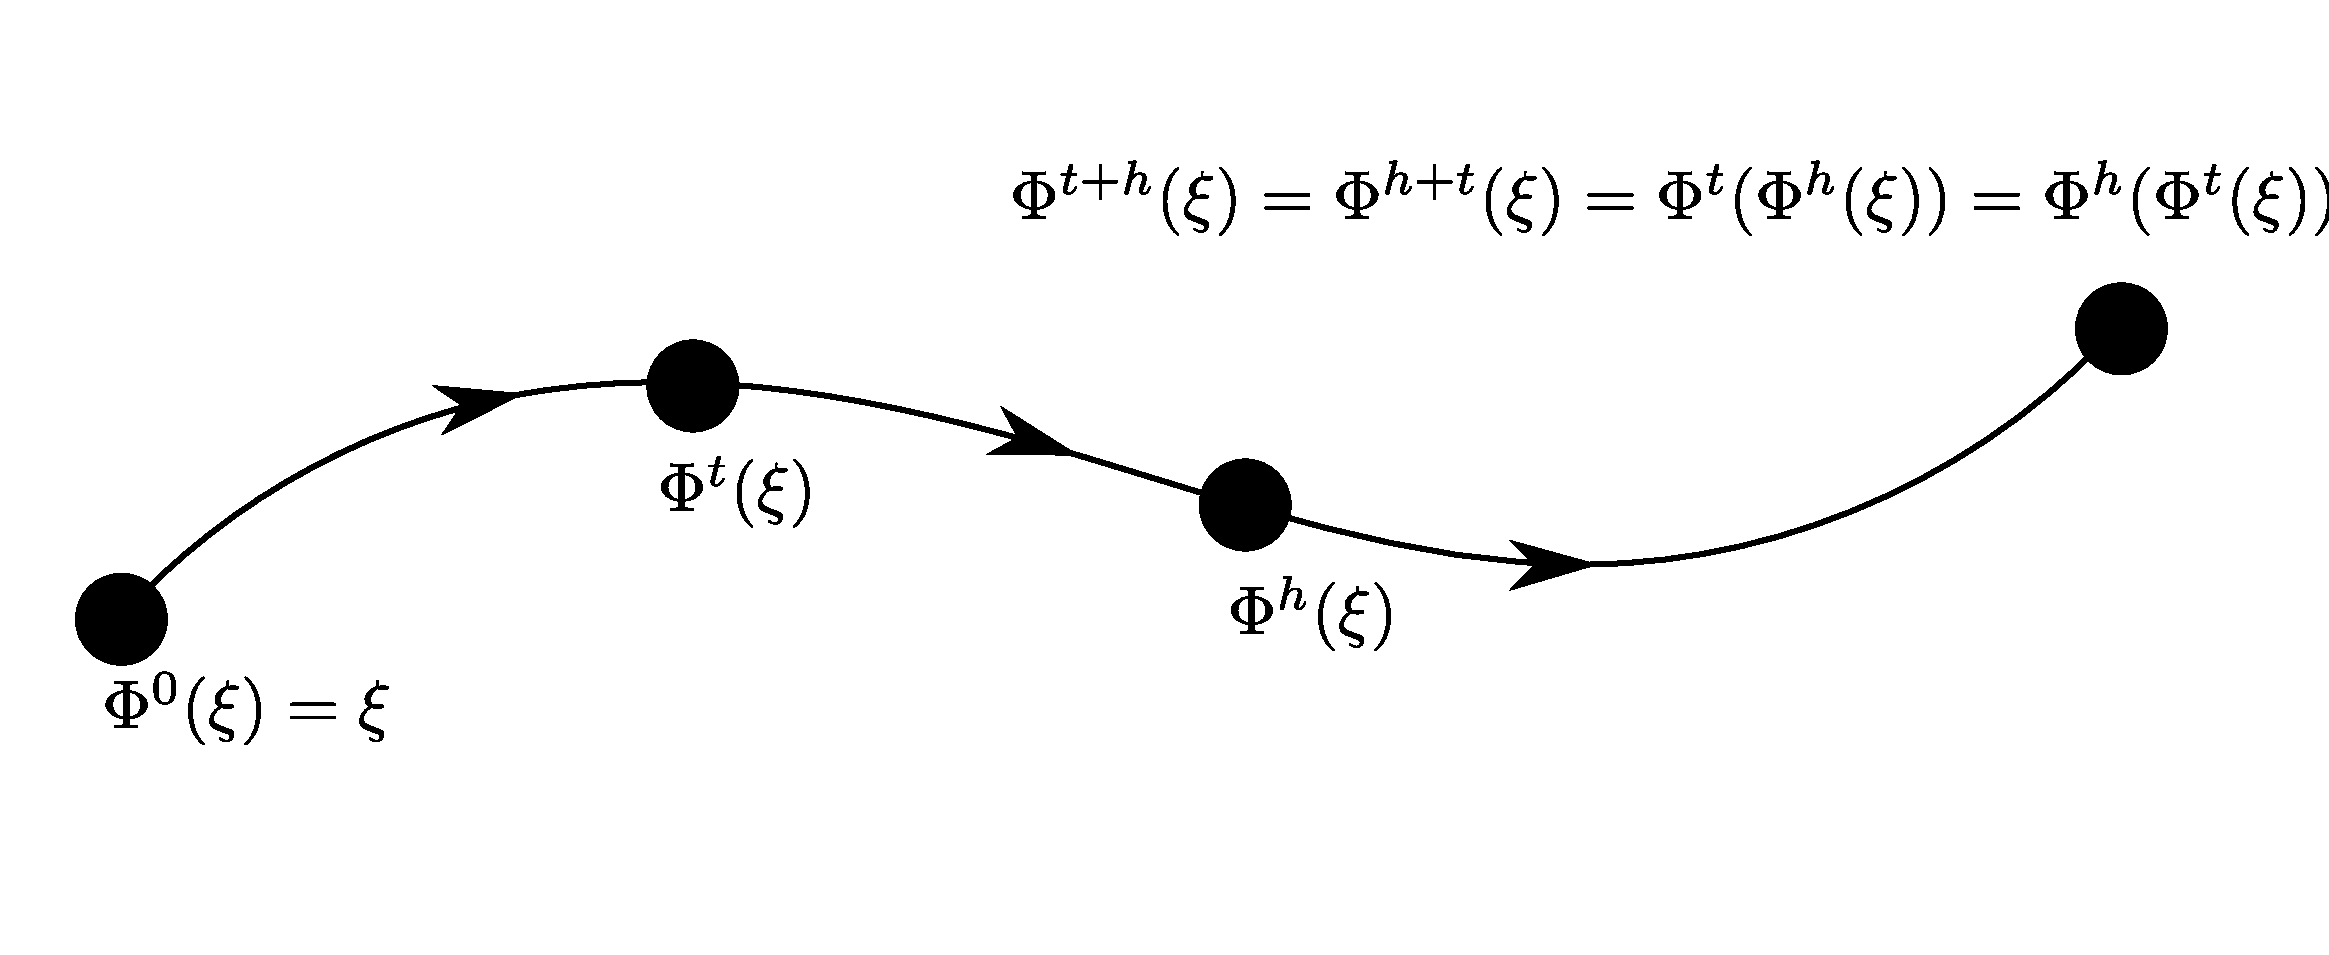
\includegraphics[width=0.75\textwidth]{images/prop.pdf}
\end{figure}

\begin{osservazione}
	$\Phi^{t_1} \circ (\Phi ^{t_2} \circ \Phi^{t_3}) = ( \Phi^{t_1} \circ \Phi{t_2}) \circ \Phi^{t_3}$, cioè "$\circ$" è associativa.
\end{osservazione}
	\item $\forall t$: se $\Phi^t$ esiste, allora esiste $(\Phi^t)^{-1}:= \Phi^{-t}$. $(x = \Phi^t (\xi) \Rightarrow \xi =(\Phi^t)^{-1}(x) )$. Per dire ciò si è sfruttato il teorema di esistenza e unicità locale di Cauchy, da cui segue che $\Phi^t$ ha proprietà di gruppo (locale). In particolare il flusso di fase è un \emph{gruppo a un parametro} di applicazioni dello spazio delle fasi in sè ($\mathbb{R}^n$, o $M$).
\end{itemize}

	\begin{adjustwidth}{1cm}{}
	\begin{mdframed}[linewidth=1.5,linecolor=purple, topline=false,rightline=false,bottomline=false]
	\textbf{Nota matematica} 
	\newline Cos'è un gruppo? $\rightarrow$ Dato un insieme G, con elementi $g \in G$, e una operazione binaria "$\circ$" (cioè l'operazione va da $G \times G$ a $G$) che gode delle seguenti proprietà:
	\begin{itemize}
	\item $g_1 \circ g_2 \in G \ \forall g_1, \ g_2 \in G$ 
	\item $g_1 \circ (g_2 \circ g_3) = (g_1 \circ g_2)\circ g_3$, $\forall g_1, g_2, g_3 \in G$ (cioè "$\circ$" è associativa).
	\item $\exists e  \in G : g \circ e = e \circ g =g \ \forall g \in G$ (esistenza dell'identità).
	\item $\forall g \in G, \ \exists \ g^{-1} \in G : g \circ g^{-1} = g^{-1} \circ g = e$ (esistenza dell'inverso per ogni elemento).
	\end{itemize}
	La coppia ($G, \circ$) si chiama gruppo (astratto).

	\begin{osservazione}
		In generale non si richiede $g_1 \circ g_2$. se questo accade ($\forall g_1, g_2 \in G$) allora il gruppo $(G, \circ)$ si dice commutativo o "Abeliano".
	\end{osservazione}
	\begin{esempio} Spazio vettoriale $\mathbb{R}^n$, con "$\circ$" = +, infatti: $e= 0(\in \mathbb{R}^n )$, $x^{-1} = -x \  \  \forall x \in \mathbb{R}^n $, e ovviamente la somma definita al solito modo (componente per componente) è associativa.
	\end{esempio}
	\begin{esempio}
		L'insieme $G$ delle natrici $n \times n$ non singolari con prodotto $\cdot$ righe per colonne ($AB$) è un esempio di gruppo non commutativo.
	\end{esempio}
	\begin{esempio}
		Le matrici ortogonali $R^TR = RR^T= \1$ sono un sottogruppo di $GL(n , \Rr)$ che si indica con $O(n)$ (gruppo ortogonale). Se si fissa $\det(R) = +1$, si ottiene $SO(n)$ (dove "S" sta per speciale).
		
		Un elementro $R \in SO(n)$ è individuato da $\frac{n(n-1)}{2}$ parametri.
	\end{esempio}
	\end{mdframed}
	\end{adjustwidth}



\newpage
\begin{teo}[Lyapunov] 
  	Sia $\overline x$ punto di equilibrio isolato di $\dot x = u(x)$. Supponiamo che esista una funzione $W: \mathbb{R}^n \rightarrow \mathbb{R}_+$ continua in $K \  \backslash \ \{\overline x \}$ tale che:
  	\begin{itemize}
  		\item $W(x) > 0 \ \ \forall x \in K \backslash  \{\overline x \}$, e $W(\overline x) =0$. Cioè W ha un minimo locale stretto in $\overline x$.
  		\item $W( \Phi^t (\xi))$ è monotona non crescente $\forall \xi \in K \backslash  \{ \overline x \}$
  	\end{itemize}
  	Ovvero una funzione di Lyapnov.
  	Allora $\overline x$ è stabile. \\ Se inoltre $W(\phi^t (\xi))$ è monotona strettamente decrescente, allora $\overline x $ è asintoticamente stabile.
  \end{teo}
  
  \begin{osservazione}
  	Nei sistemi meccanici spesso/quasi sempre, la funzione $W$ è l'integrale di Jacobi/energia del sistema. Infatti $H$ ha un minimo nei punti di equilibrio stabili, invece quando si ha l'attrito, gli stessi equilibri stabili si trasformano in asintoticamente stabili, infatti $H$ diminuisce monotonamente lungo il moto. Per avere un'intuizione basta pensare al caso dell'oscillatore semplice con e senza attrito, nel primo caso attorno all'equilibrio si aprono delle ellissi, nel secondo caso delle spirali che tendono al punto $(0,0)$. Nei casi non meccanici l'idea è comunque quella di cercare un integrale primo del sistema e valgono praticamente le stesse considerazioni.
  \end{osservazione}


\begin{dm}

Sia $J \subset K$ intorno di $\overline x$ e sia $\alpha := \ \underset{x \in \partial J}{min} \ W(x)>0$. Si definisce l'insieme l'insieme

\begin{equation}
  G:= \{ x \in J : W(x) < \alpha \}
\end{equation}

\begin{figure}[H]
    \centering
  \includegraphics[width=0.5\textwidth]{images/teoremaLyapunov.pdf}
\end{figure}


Intanto $G$ non è vuoto perché
$$
\overline x \in G: \ \ W ( \overline x)=0< \alpha
$$
\\
La funzione $\alpha - W(x)$ è \textbf{continua ed è $>0$ in $\overline x$} 

$\Rightarrow$ [Teorema permanenza del segno] cioè $\exists I $ di $\overline x$ tale che $\alpha - W(x)>0$ con $I \subseteq G$. 

L'insieme G è $\Phi^t $ - invariante: preso $\xi \in G \Rightarrow \Phi^t(\xi) \in G \ \ \forall t \geq 0$. Infatti se $W(\xi) < \alpha \  (\xi \in G)$ (definizione di $G$), allora $W(\Phi^t(\xi)) \leq W (\xi) < \alpha$, dove la prima disequazione è la seconda ipotesi del teorema.
Ma allora $\forall \xi \in I \subseteq G \subseteq J \Rightarrow \Phi^t (\xi)$ non esce da G e quindi da J. E quindi $\overline x$ è stabile.
\bigskip\\
Segue ora la seconda parte del teorema. Quindi sfruttando la terza ipotesi ovvero che $W(\Phi^t(\xi))$ sia monotona decrescente $\forall t \geq 0$, $\forall \xi \in K \backslash \{\overline x \}$.
Dato $\lim_{t \rightarrow +\infty} \Phi^t (\xi) = \overline x$, per la definizione di limite si ha $\forall t>t_L$ tale che $t$ appartiene ad un intorno di $t_L$, $ \exists \hat{L} $, intorno di $\overline x$, tale che vale $\Phi^t ( \xi) \in \hat{L} $. Quindi la funzione è inferiormente limitata.\\
    Supponendo ora per assurdo che $\lim_{t \rightarrow +\infty} \Phi^t (\xi) \neq \overline x$, ovvero si nega la definizione precedente: $\Phi^t (\xi) \notin \hat{L} ~ \forall t > t_L$.\\
	È noto che $W\mid_{\partial \hat L}$ assume max e min (teorema di Weierstrass). Chiamando $\beta= \underset{x \in \partial \hat L}{\text{min}} W(x)$.\\
	Poiché $W(\Phi^t(\xi)) \rightarrow 0 $, esiste $T_\beta$ tale che $W(\Phi^t(\xi)) < \beta$ per $t >T_\beta$.\\
	Ma dall'altra parte $\exists t^*_L>T_\beta$ tale che a $t=t_L^*$, $\Phi^t (\xi) \in \partial \hat L $ $\Rightarrow W (\Phi^{t^*_L}(\xi)) \geq \beta$.\\ Questa è la contraddizione cercata, cioè non esiste nessun $\hat L$ con la proprietà cercata e quindi $\overline x$ è asintoticamente stabile.
\end{dm}

Per sistemi meccanici naturali conservativi la lagrangiana è
\begin{gather}
	\L = \K_2 - \U = \frac{1}{2} \dot q \cdot A(q) \dot q - \U(q)
\end{gather}
Si conserva $H= \K_2 + \U(q)$. Sia $\bar q$ un punto di minimo locale stretto $\U(q)$, definendo $W(q,v):=H(q,v)- H(\bar q, 0)$ la funzione di Lyapnov, tale per cui è 0 nel punto di equilibrio, esplicitamente si ha
\begin{gather}
	W(q,v):=H(q,v)- H(\bar q, 0) = \frac{1}{2} v \cdot A(q) v + \U(q) - \U(\bar q)
\end{gather}

\newpage
\begin{osservazioni}
	\item Si può notare che
	\begin{equation*}
	W(q,v)\begin{cases}
		=0 	\ &\text{in } \vec{\bar q \\ 0} \\
		>0 \ &\forall \vec{q \\v} \neq \vec{ \bar q \\ 0} \ \text{in un opportuno intorno $B$ di} \ \vec{\bar q \\ 0}
	\end{cases}
\end{equation*}

\item 
\begin{gather}
	W( \Phi^t (q,v)) = H( \Phi^t (q,v)) - H(\bar q,0)=\\
	=H(q,v) - H(\bar q,0) = W(q,v)
\end{gather}

$\Rightarrow \vec{\bar q \\ 0}$ è stabile secondo Lyapnov

\item In generale se W è di classe $C^1(K \backslash \{ \overline x \})$ la seconda proprietà del teorema è soddisfatta se 
$\dot W = \frac{d}{dt}W (\Phi^t (\xi)) \leq 0 \ \ \forall t \geq 0 \ \ \forall \xi \in K \backslash \{ \overline x \}$.
\begin{gather}
	\frac{d}{dt}W ( \phi ^t (\xi ))= \frac{d}{dt}( W (x_1 (t),...,x_n(t))=\\
	= \sum_{j=1}^n \frac{ \partial W}{\partial x_j} \dot x_j = \sum_j \frac{ \partial W}{\partial x_j} u_j (x)=\\
	= (u \cdot \nabla W)(\Phi^t (\xi))= u (\Phi ^t (\xi)) \cdot \nabla W (\Phi ^ t(\xi))
\end{gather}
Dove $u \cdot \nabla W$ è la derivata nella direzione di $u$  o anche derivata di Lie di $W$ lungo il flusso del campo vettoriale $u$.

Se $\dot W = \frac{d}{dt}W (\Phi^t (\xi)) < 0$ segue la terza proprietà del teorema cioè la stabilità asintotica.

\end{osservazioni}





\newpage
\renewcommand{\tem}{$\L$}
\begin{tema}[Moto armonico smorzato]
\begin{equation}\label{smorzato}
m \ddot x = -kx - \gamma \dot x
\end{equation}
Definisco $\omega^2:= \frac{k}{m}$ e $2 \mu := \frac{\gamma}{m}>0$
$$
\ddot x = - \omega^2 x - 2 \mu \dot x
$$
$$
\iff \begin{cases}
	\dot x = v\\
	\dot v= -\omega^2 x - 2 \mu v
\end{cases}
$$
Quindi la parte di destra è $\vec 0$ soltanto per l'equilibrio $(x,v)=(0,0)$.\\
Essendo l'equazione originale un'equazione diff. scalare lineare di secondo ordine a coefficienti costanti, possiamo usare i metodi di analisi 3 per la soluzione esplicita: sostituiamo $x(t)= e^{\lambda t}$ nell'equazione di partenza per trovare gli autovalori della matrice $A$ dell'equazione differenziale messa al primo ordine. Vediamone una breve dimostrazione. Vogliamo mostrare che si $\lambda$ ottengono così 
$$
\ddot x + 2 \mu \dot x + \omega^2 x =0= e^{\lambda t} \underbrace{(\lambda^2 + 2 \mu \lambda + \omega^2}_{=0} )
$$
sono proprio gli autovalori di $A$ dove $A$ è:
$\left( \begin{array}{c}
 \dot x \\ \dot v
 \end{array} \right)  =  \underbrace{\left(  \begin{array}{c}
 	0 \ \ \ \ \ \ \ \ \ \ \ 1 \\ -\omega^2 -2 \mu \end{array} \right)  }_{A} 
  \left( \begin{array}{c}
 	x \\ v
 \end{array} \right)  = A \left( \begin{array}{c}
 	x \\ v
 \end{array} \right) $
E se è verificata la condizione che abbiamo scritto sopra, cioè prendiamo le soluzione del tipo esponenziale con esponente ottenuto nel modo indicato abbiamo:
 $$
 \left( \begin{array}{c}
 x \\ v
 \end{array} \right)  = u e^{\lambda t} \ \ \ \ u \in \mathbb{R}^2 \longrightarrow \lambda\cancel{e^{\lambda t}}= A u \cancel{e^{\lambda t}}
 $$
 $$
 \Rightarrow Au = \lambda u
 $$
 $$
 Au = \lambda u  \iff (A - \lambda \1)u=0
 $$
 soltanto se la matrice di sinistra è non invertibile (cioè rango non massimo) che esistono $u( \neq 0$) che risolvono l'equazione appena scritta. Ed è soltanto in questo caso che ha senso cercare soluzione del tipo $u e^{\lambda t}$. Infatti se la matrice di sinistra fosse invertibile:
 $$
 \text{se det} (A-\lambda \1) \neq 0 \Rightarrow \cancel{(A-\lambda \1)^{-1}(A-\lambda \1)}u=0
$$

 $$
 \Rightarrow u \equiv 0
 $$
Quindi imponiamo che la matrice sia di rango non massimo:
 $$\exists \ u \neq 0 \iff det(A- \lambda \1)=0$$
Da cui sviluppando l'ultimo determinante abbiamo:
 $$det(A-\lambda \1)= \lambda^2 + 2 \mu \lambda + \omega^2=0$$
che è quello che volevamo mostrare.\\
In questo caso i due autovalori risultano:
 $$
 \lambda_\pm = - \mu \pm \sqrt{\mu^2 -\omega^2}
 $$
 Possiamo fare una classificazione in base alla natura di tali autovalori:
  \begin{immagine}
 	{trees.pdf}{}
 \end{immagine}
 \begin{enumerate}
 	\item \textbf{Autovalori reali}: $\mu > \omega \Rightarrow \lambda_- < \lambda_+<0$ \textit{caso "sovrasmorzato"}, in questo caso l'agente dissipativo fa si che non avvengano oscillazioni, infatti le soluzioni, come detto prima, sono combinazioni lineari di $e^{\lambda_+ t}$ e $e^{\lambda_- t}$:
 	$$
x(t)= a e^{\lambda_+t} + b e^{\lambda_-t}
$$
che per $\lambda$ reali (negativi) è evidentemente monotona e decresce esponenzialmente:
$\lim_{t \rightarrow + \infty} x(t)=0 \ \ \ \ (\forall \ a,b,$ cioè $\forall$ dato iniziale \ con $(a,b) \neq 0 )$.
 \begin{immagine}
 	{sovrasmorzato.pdf}{}
 \end{immagine}
 


 	\item $\mu = \omega \Rightarrow \lambda :=\lambda_- = \lambda_+=-\mu$ \textit{ caso con smorzamento critico}\\
 	Sebbene il sistema sia in grado di dare inizio alla prima oscillazione, la vede smorzarsi completandola solo all'infinito. Le soluzioni generali sono combinazioni lineari di $e^{\lambda t}$ e $te^{\lambda t}$.
 	\begin{immagine}
 	{smorzamentocritico.pdf}{}
 	\end{immagine}
 	\item $\mu< \omega \Rightarrow \overline \lambda_- = \lambda_+ = -\mu + i \sqrt{\omega^2 - \mu ^2}$ \textit{caso "sotto smorzato"}\\
 	La soluzione generale è come prima la combinazione lineare di $e^{\lambda_+ t}$ e $e^{\lambda_- t}$ e dalla formula di Eulero si deduce che è ora presente una componente ondulatoria. Siamo interessati soltanto alla parte reale/fisica della soluzione che si scrive decomponendo in parte reale e in parte immaginaria e prendendo quella reale:
 	$$
 	x(t) = a_+ e^{\lambda_+t} + a_- e ^{\lambda_- t}, \ \ \ \overline a_- =a_+
 	$$
 	$$
	=a_+ e^{\lambda_+t} + \overline{a}_+ e^{\overline{\lambda}_+t} = a_+ e^{\lambda_+ t} + (\overline{a_+ e^{\lambda_+t}})
	$$
	$$
	=(a_+' +i a_+'')e^{(- \mu + i \sqrt{\omega^2 - \mu^2})t} + (a_+' - i a_+'')e^{(- \mu - i \sqrt{\omega^2 - \mu^2})t}
	$$
	$$
	=e^{-\mu t} [ a_+' ( e^{i \sqrt{\omega^2 -\mu ^2 }t} + e^{-i \sqrt{\omega^2 \mu^2}t}) + a_+'' i (e^{i \sqrt{\omega^2 - \mu^2}t}- e^{-i \sqrt{\omega^2 -\mu^2}t})]
	$$
	Usando le formule di Eulero: $e^{i \theta}= \cos \theta + i \sin \theta$.
	$$
	=e^{-\mu t} [\underbrace{2a_+}_a \cos (\sqrt{\omega^2 -\mu^2}t) \underbrace{-2a_+''}_b \sin (\sqrt{\omega^2 -\mu^2}t)]
	$$
	$$
	=e^{-\mu t}[a \cos (\sqrt{\omega^2 -\mu^2}t) + b \sin (\sqrt{\omega^2 -\mu^2}t)]
	$$
	Studiando il comportamento per $t\rightarrow + \infty$ trovo $\lim_{t \rightarrow + \infty} x(t)=0 \ \ \ \  (\forall \ a,b,$ cioè $\forall$ dato iniziale \ con $(a,b) \neq 0 )$..\\
	 \begin{immagine}
 	{sottosmorzato.pdf}{}
 \end{immagine}
 

 \end{enumerate}
Dopo vedremo una generalizzazione di questo procedimento con autovalori per decidere la natura di un punto di equilibrio.\\
Qual è invece la funzione di Lyapunov del sistema? Nonostante non sia conservativo è ancora l'energia totale del sistema (con una piccola precisazione), infatti presenta un minimo locale stretto nel punto di equilibrio $(x,v)=(0,0)$ e lungo il flusso non solo è non crescente, ma è addirittura  strettamente decrescente:

\begin{gather}
   H(x,v) := \frac{mv^2}{2} + \frac{kx^2}{2}\\
 \frac{d}{dt}H(\underbrace{x(t),v(t)}_{\Phi^t(x_0,v_0)}) =\pp{H}{x} \dot x + \pp{H}{v} \dot v=\\=
  k xv + mv \left( - \frac{kx}{m} - \frac{\gamma v}{m} \right)=\\
= - \gamma v^2
\end{gather}

di conseguenza $H$ è non crescente lungo il flusso (quindi $(0,0)$ è stabile), ma siccome non è vero che $H$ è strettamente decrescente si può concludere immediatamente che il punto in questione sia anche asintoticamente stabile. Però nonostante la derivata di $H$ si annulli in punti del tipo $(x,0)$, ma sono soltanto delle valli (lungo il flusso) per la funzione $H$. Infatti il campo di velocità nel piano delle fasi $(x,v)$ calcolato nei punti $(x,0)$ risulta trasversale alla varietà $v=0$, e quindi il moto nel piano delle fasi non si ferma mai: se si raggiunge in un punto del tipo $(x,0)$ si viene spinti via cosicchè il moto tende comunque nel punto $(0,0)$. più rigorosamente il campo vettoriale del sistema è:

\begin{equation}
  \left.
\left( \begin{array}{c}
v \\ -\frac{k}{m}x - \frac{\gamma}{m}v
\end{array} \right)  \right|_{\underbrace{v=0}_{asse \ x}}  = \left( \begin{array}{c}
 0 \\ - \frac{k}{m}x
 \end{array} \right)
\end{equation}
 
Quello che si vuole mostrare è che, anche se $\dot H=0$ sull'asse $x$, il moto non resta poi "intrappolato" sull'asse $x$, bensì $H$ ricomincia a diminuire fino a far spiraleggiare $x$ sull'origine. A quel punto è eliminato il dubbio sul moto introdotto da $\dot H=0$ e si può concludere che $(0,0)$ è equilibrio asintoticamente stabile.
Infatti studiando la struttura del campo vettoriale, si vede che se $x>0$, i vettori ortogonali all'asse x rimpiccioliscono, fino a diventare uguali a 0 sull'origine; stesso ragionamento per $x<0$.
\end{tema}


\subsection{Linearizzazione}

\begin{gather}
	H= \K_2 + \U(q) + \U( \bar q)
\end{gather}
Sviluppando $H(q,v)$ attorno a $(\bar q , 0)$ secondo Taylor fino all'ordine sue con $q= \bar q + \xi$ si ha 
\begin{gather}
	H( \bar 	 q+ \xi, v) = \frac{1}{2} v \cdot A ( \bar q )  v + \frac{1}{2} \xi \cdot \pp{^2 \U}{q^2} (\bar q) \xi +o(3)
\end{gather}
Into a $(\bar q,0)$, passando dalle coordinate $\xi$ a $c$, cioè quelle per cui $\xi = \sum_i c_i u_i$, l'espansione diventa
\begin{gather}
	H= \sum_i^L \left( \frac{\dot c_i^2}{2} + \frac{\omega_i^2}{2} c_i^2 \right) + o(3)= \Delta E
\end{gather}
Questa è l'energia di scarto rispetto al minimo, perchè il minimo è stato sottratto. Se non si considera il resto si ha l'equazione di un ellissoide immerso in uno spazio di dimensione $2L$:
\begin{gather}
	 \sum_i^L \left( \frac{c_i^2}{2 \Delta E /\omega_i^2} + \frac{\dot c_i^2}{2 \Delta E}  \right) =1
\end{gather}



\newpage
\section{Esercizi} \toc
\begin{tema}[Pendolo doppio]
L'idea grafica del problema è:

\begin{figure}[H]
    \centering
 \includegraphics[width=0.5\textwidth]{images/pendolodoppio}
\end{figure}
La condizione del perno è
\begin{gather}
	x_1^2 + y_1^2= r ^2
\end{gather}
Per quanto riguarda il punto alla fine del pendolo esso si può muovere lungo una circonferenza di raggio $r$ centrata sul perno, quindi:
\begin{gather}
	(x_2-x_1)^2 + (y_2-y_1)^2 = r^2
\end{gather}
\subsubsection*{Parametrizzazione}
Ci si aspetta che la varietà vincolare $\M$ sia una varietà prodotto di due cerchi. Questo vuol dire che $\M = \S^1 \times \S^2 := \Pi^2$. Per definizione il prodotto di due cerchi è un toro. 

\begin{figure}[H]
    \centering
  \includegraphics[width=0.5\textwidth]{images/toro}
\end{figure}

Allora le coordinate libere, lagrangiane, sono $\theta_1$ e $\theta_2$ e si può quindi scrivere
\begin{gather}
	x_1 = r \sin \theta_1 \\
	y_1 = - r \cos \theta_1\\
	x_2 = x_1 + r \sin \theta_2 = r (\sin \theta_1 + \sin \theta_2)\\
	y_2 = x_2 - r \sin \cos \theta_2 = -r ( \cos \theta_1 + \cos \theta_2)
\end{gather}
\subsubsection*{Forma della lagrangiana}
L'energia cinetica $\K$ si calcola come 
\begin{gather}
	\K = \frac{m}{2} \left. (\dot x_1^2 + \dot y_1^2  + \dot x_2^2 + \dot y_2^2 ) \right|_\M = \\=\frac{m r^2}{2} \left [\dot \theta ^2_1 + \dot \theta_1 ^2 +(\dot \theta_1 \cos \theta_1 + \dot \theta_2\cos \theta_2)^2 + ( \dot \theta_1 \sin \theta_1 + \dot \theta_2 \sin \theta_2)^2 \right]=\\
	= \frac{mr^2}{2} \left[ \dot \theta^2_1 + \dot \theta^2_1 + \dot \theta^2 _2 + 2 \dot \theta_1 \dot \theta_2 ( \cos \theta_1 \cos \theta_2 + \sin \theta_1 \sin \theta_2 ) \right] =\\
	= \frac{m r^2}{2} [ 2 \dot \theta_1^2 + \dot \theta_2^2 + 2 \dot \theta_1 \dot \theta_2 \cos ( \theta_1 - \theta_2)]=\\
	= mr^2 \frac{1}{2} (\dot \theta_1, \dot \theta_2) \underbrace{\left( \begin{matrix}
		2 & \cos (\theta_1- \theta_2) \\ \cos (\theta_1-\theta_2) &1
	\end{matrix} \right)}_{A(\theta)} \vec{\dot \theta_1 \\ \dot \theta_2 }
\end{gather}
	
L'energia potenziale è della forma
\begin{gather}
	\U(\theta) = \left. U \right|_\M =\left. mgy_1 + mgy_2 \right|_\M=\\
=-mgr \cos \theta_1 - mg r ( \cos \theta_1 + \cos \theta _2)=\\
=- mgr ( 2 \cos \theta _1 + \cos \theta _2)	
\end{gather}	
Allora la lagrangiana è della forma
\begin{gather}
	\L (\theta, \dot \theta) = \K -\U = \\
	= \frac{mr^2}{2} \dot \theta \cdot A(\theta) \dot \theta + mgr ( 2 \cos \theta_1 + \cos \theta_2)
\end{gather}
Le equazioni del moto saranno date da
\begin{gather}
	\dd{}{t} \pp{\L}{\dot \theta_1} - \pp{\L}{\theta_1} =0 \\
	\dd{}{t} \pp{\L}{\dot \theta_2} - \pp{\L}{\theta_2} =0 
\end{gather}
Si può ridurre la scrittura della lagrangiana nel seguente modo
\begin{gather}
	mr^2 \L ' = mr^2 \left[ \frac{1}{2} \dot \theta \cdot A(\theta) \dot \theta + \omega^2 _0 (2 \cos \theta_1 + \cos \theta_2) \right], \ \ \omega _0=\sqrt{\frac{g}{r}}
\end{gather}	
L'energia del sistema è
\begin{gather}
	H(\theta, \dot \theta) = \K' + \U' = \frac{1}{2} \dot \theta \cdot A(\theta) \dot \theta - \omega_0^2 ( 2 \cos \theta_1 + \cos \theta_2)
\end{gather}

\subsubsection*{Equilibri}
\begin{equation}
	\nabla_\theta \ \U'(\theta) =0 
\end{equation}
Che è equivalente al sistema
\begin{gather}
	\begin{cases}
		\pp{\U'}{\theta_1} =0 \\
		\pp{\U'}{\theta_2}=0 
	\end{cases} \Rightarrow \begin{cases}
 	2 \omega_0^2 \sin \theta_1 = 0\\
 	\omega^2_0 \sin \theta_2 =0
 \end{cases} \Rightarrow \begin{cases}
 	\theta_1 =0, \pm \pi\\
 	\theta_2 =0 , \pm \pi
 \end{cases}
\end{gather}
Avendo definito la varietà $\M= \S \times \S$ non tutti questi valori sono ammessi, bensì
\begin{gather}
	\theta_1 \in ] - \pi , \pi] , \ \theta _2 \in ] \- \pi , \pi]
\end{gather}
Ci sono allora 4 equilibri 
\begin{gather}
	\vec{\theta_1 \\ \theta_2} = \underbrace{ \vec{0 \\ 0}}_{1} , \underbrace{ \vec{\pi \\ \pi}}_{2} , \underbrace{\vec{ 0 \\ \pi} }_{3} , \underbrace{\vec{ \pi \\ 0} } _4
\end{gather}
\begin{figure}[H]
    \centering
  \includegraphics[width=0.5\textwidth]{images/equilibri}
\end{figure}

\subsubsection*{Stabilità}
Si calcola l'hessiano
\begin{gather}
	\pp{^2 \U}{\theta^2} = \left(\begin{matrix}
		\pp{^2 \U'}{\theta_1^2} & \pp{^2 \U'}{\theta _2 \partial \theta_1} \\  \ \\
		\pp{^2 \U' }{\theta_1 \partial \theta_2} & \pp{^2 \U'}{\theta_2^2}
	\end{matrix}\right) = \left( \begin{matrix}
		2 \omega_0^2 \cos \theta_1 & 0 \\ 0 & \omega_0 ^2 \cos \theta_2
	\end{matrix} \right)\\
	\pp{^2}{\theta^2} (0,0) =  \underbrace{ \left(\begin{matrix}
		2 \omega_0^2 & 0 \\ 0 & \omega_0^2
	\end{matrix} \right)}_{\bar B}
\end{gather}
Che è definita positiva e quindi è un punto di minimo non degenere e, siccome l'energia è una funzione di Lyapnov, è anche stabile secondo Lyapnov. Gli altri punti invece sono instabili.


Adesso si diagonalizzano simultaneamente la matrice cinetica (di massa) e potenziale nei punti di equilibrio:
\begin{gather}
	\bar A := A(0,0) = \left.\left( \begin{matrix}
		2 & \cos (\theta_1- \theta_2) \\
		\cos (\theta_1- \theta_2) & 1 
	\end{matrix} \right) \right|_{\theta_1=\theta_2=0} = \left( \begin{matrix} 2 & 1 \\ 1 & 1 \end{matrix} \right)\\
	\bar B:= \pp{^2 \U'}{\theta^2} (0,0) = \left( \begin{matrix} 2 \omega_0^2 & 0 \\ 0 & \omega_0^2 \end{matrix} \right)
\end{gather}
Si può ora calcolare la lagrangiana espansa all'ordine 2 attorno al punto di equilibrio nello spazio delle fasi
\begin{gather}
	\Rightarrow \L _2= \frac{1}{2} \dot \theta \cdot \bar A \dot \theta - \frac{1}{2} \theta \cdot \bar B \theta=\\ = \frac{1}{2} ( \dot \theta_1, \dot \theta_2) \left( \begin{matrix}
		2 & 1 \\ 1 & 1
	\end{matrix} \right) \vec{\dot \theta_1 \\ \dot \theta_2} - \frac{1}{2} ( \theta_1, \theta_2) \left( \begin{matrix}
		2 \omega_0^2 & 0 \\ 0 & \omega_0^2 
	\end{matrix}\right)  \vec{ \theta_1 \\ \theta_2} = \\
	= \frac{1}{2} (2 \dot \theta_1^2 + \dot \theta^2_2 + 2 \dot \theta_1 \dot \theta_2 ) - \frac{\omega_0^2}{2} ( 2 \theta_1^2 + \theta_2^2)
\end{gather}

\subsubsection*{Frequenze proprie}
Sono date dalla soluzione di 
\begin{gather}
	\det (\omega^2 \bar A - \bar B )=0\\
	\det \left[\left( \begin{matrix}
		2 \omega^2 & \omega^2 \\ \omega^2 & \omega^2
	\end{matrix} \right) - \left( \begin{matrix}
		2 \omega_0^2 & 0 \\ 0 & \omega_0^2
	\end{matrix} \right)\right] =\\
	= \det \left( \begin{matrix}
 	2(\omega^2- \omega_0^2) & \omega^2 \\ \omega^2 & \omega^2 - \omega_0^2
 \end{matrix} \right)=\\
 = 2 (\omega^2 - \omega_0^2)^2 - \omega^4 = \omega^4 - 4 \omega_0 ^2 \omega^2 + 2 \omega_0^4=\\
 \omega_\pm^2 = 2 \omega_0 ^2 \pm \sqrt{4 \omega_0 ^4 - 2 \omega_0 ^4}= \omega_0^2 \left( 2 \pm \sqrt{2}\right)\\
 \ \\
 \Rightarrow \boxed{\omega_\pm = \omega_0 \sqrt{2 \pm \sqrt{2}}}
\end{gather}
\subsubsection*{Vettori propri}
Si cercano adesso i vettori propri $u^+ $ e $u^-$ che soddisfano
\begin{gather} 
	( \omega_+ ^2 \bar A - \bar B ) u^+ =0 \iff \left( \begin{matrix}
 	2(\omega_+^2- \omega_0^2) & \omega_+^2 \\ \omega_+^2 & \omega_+^2 - \omega_0^2
 \end{matrix} \right) \vec{ u_1^+ \\ u_2^+} = \vec{0 \\ 0}\notag  \\
 \overset{\text{1 eq.}}{\longrightarrow} 2 \omega_0^2 (1+ \sqrt{2} ) u_1^+ + \omega_0^2 ( 2+ \sqrt{2} ) u_2^+=0\\
 2\cancel{ (1+ \sqrt{2} )}u^+_1  \sqrt{2} \cancel{ (1+ \sqrt{2} )} u_2^+ =0\\
 	\boxed{\sqrt{2} u_1^+ + u_2^+=0}
\end{gather}
Per l'altro vettore si ha
\begin{gather}
	( \omega_+ ^2 \bar A - \bar B ) u^- =0 \iff \left( \begin{matrix}
 	2(\omega_-^2- \omega_0^2) & \omega_-^2 \\ \omega_-^2 & \omega_-^2 - \omega_0^2
 \end{matrix} \right) \vec{ u_1^- \\ u_2^-} = \vec{0 \\ 0}\notag  \\
	2 \cancel{\omega_0^2} (1- \sqrt{2}) u_1^- + \cancel{\omega_0^2} (2- \sqrt{2}) u_2^- =0\\
	\boxed{\sqrt{2} u_1^- - u_2^-=0}
\end{gather}
Allora come vettori propri, fissando per ogni vettore una componente, si ha
\begin{gather}
	u^+ = \vec{ 1 \\ \sqrt{2} }, \ u^- = \vec{1 \\ \sqrt{2}}
\end{gather}
	
\end{tema}


\begin{esercizio}
	Ripetere il tema del pendolo doppio imponenddo $\theta_1=\theta_2 = \theta$
	\begin{enumerate}
		\item Scrivere la lagrangiana
		\item Determinare le posizioni di equilibrio
		\item Studiare le piccole oscillazione attorno al punto di equilibrio stabile, in particolare la loro frequenza
	\end{enumerate}
\end{esercizio}

\begin{tema}[Pallina che rotola sul fondo]
	Lo schema mentale che si fa quando si pensa a un minimo di potenziale è una pallina che rotola in fondo a una buca, in questo esempio si verificherà se l'idea generalizzata è fondata per una dimensione. Quindi si studia una massa m, pesante, vincolata su una curva piana. La quota è assegnata da una funzione delle coordinate $x$, $y=h(x)$.
\begin{figure}[H]
    \centering
  \includegraphics[width=0.5\textwidth]{images/hx}
\end{figure}


Innanzitutto l'energia potenziale è data da
\begin{gather}
	\U = \left. mgy \right|_\M = mgh(x) 
\end{gather}
Invece l'energia cinetica è data da 
\begin{gather}
	\K = \frac{m}{2} \left. (\dot x^2 + \dot y^2) \right|_\M = \\
	= \frac{m}{2} ( 1+ (h'(x) )^2) \dot x^2
\end{gather}
La lagrangiana e l'energia sono allora 
\begin{gather}
	\L = \K -\U = \frac{m}{2} ( 1+ (h'(x))^2)\dot x^2 - mg h(x)\\
	H(x, \dot x) = \K + \U = \frac{m}{2} ( 1 + (h'(x))^2)\dot x^2 + mg h(x)
\end{gather}
Vale la conservazione dell'energia $\K +\U=E \rightarrow \K = E-\U(x)\geq 0$.
In generale si può vedere che a meno del fattore $h'(x)$ vale che l'approssimazione di una funzione qualsiasi come una pallina che scorre vicino a un minimo è vera, la $\U$ invece agisce solo come un riscalamento dell'energia.

\begin{figure}[H]
    \centering
  \includegraphics[width=0.6\textwidth]{images/h(x)}
\end{figure}

Studiando le piccole oscillazione attorno a un punto di minimo locale non degenera bisogna determinare 
\begin{gather}
	\bar x: \U' (\bar x ) = 0 \iff h'( \bar x) =0 \\
	\U''( \bar x) = mg h'' ( \bar x) >0
\end{gather}
La lagrangiana espansa fino all'ordine 2 è allora
\begin{gather}
	\L_2 = \frac{m}{2} ( 1+ (h' (\bar x))^2)\dot \xi^2 -mg \left(h(\bar x)+ h'(\bar x) \xi + \frac{1}{2} h"(\bar x) \xi^2\right)\\
	\boxed{h'(\bar x)=0 } \Leftarrow \text{ condizione di minimo}\\
	= \frac{m}{2} \dot \xi^2 - \frac{mg}{2} h''(\bar x)\xi^2 \cancelto{\text{è un riscalamento}}{-mgh(\bar x)}=\\
	\ \notag \\
	\Rightarrow \boxed{\dd{}{t}\pp{\L_2}{\dot \xi}= \pp{\L_2}{\xi} \iff \cancel{m} \ddot \xi = - \cancel{m} g h''(\bar x) \xi \Rightarrow \omega:= \sqrt{g h''(\bar x)}}
\end{gather}
La forma della lunghezza di un tratto della curva $h(x)$ è dato da 
\begin{gather}
	s(x) = \int_{\bar x}^ x \sqrt{1 + (h'(x))^2}dx\\
	\dot s(x(t))= \sqrt{1+ (h'(x))^2} \dot x
\end{gather}
È possibile esprimere la lagrangiana come funzione di $s$ e $\dot s$ ovvero
\begin{gather}
	\L(s, \dot s) = \frac{m \dot s^2}{2} - mg\underbrace{h \overset{\overset{\text{invertendo}}{\uparrow}}{(x(s))}}_{\tilde h(s)}=\\
	= \frac{m \dot s^2}{2} - mg \tilde h(s)
\end{gather}
In questo modo si è ottenuto un'espressione facile per l'energia cinetica ma difficile per il potenziale sfruttando l'invarianza della lagrangiana per qualsiasi cambio di coordinate.
\end{tema}

\newpage
\begin{tema}[Pallina su anello rotante]
	Il sistema è costituito da una massa vincolata a muoversi su un cerchio rotante. 
	
	\begin{figure}[H]
    \centering
  \includegraphics[width=0.5\textwidth]{images/pendolosferico.pdf}
\end{figure}
	

	
	L'equazione della varietà vincolare si può trovare in diversi modi, eccone tre
	\begin{enumerate}
		\item Si nota innanzitutto che l'asse $\hat z$ rimane lo stesso quando l'anello ruota. Le posizioni allora sono
		\begin{gather}
			x(t) = X(t) \cos \omega t\\
			y(t) = X(t) \sin \omega t
		\end{gather}
		Dove $X(t)$ è la posizione dell'asse X solidale all'anello ad ogni tempo t che sarà legato alla forma dell'anello come $X(t)= R \sin \theta (t)$. Quindi
		\begin{gather}
			\begin{cases}
				x(t) = R \sin \theta(t) \cos \omega t \\
				y(t) = R \sin \theta(t) \sin \omega t \\
				z(t) = R\cos \theta (t)
			\end{cases}
		\end{gather}
		\item Si deduce che tale trasformazione di coordinate fare una rotazione del tipo
		\begin{gather}
			\vec{x(t) \\ y(t) \\ z(t)} = \left( \begin{matrix} 
 	\cos \omega t & - \sin \omega t & 0 \\ \sin \omega t & \cos \omega t & 0 \\ 0 & 0 & 1
 \end{matrix}\right)\vec{X(t) \\ Y(t) \\ Z(t)}
		\end{gather}  
		
		\item Si può immaginare, grazie alla simmetria sferica del problema, che il punto sia descrivibile con coordinate sferiche di angolo polare $\varphi(t)=\omega t$.
	\end{enumerate}
	Allora si ha che 
	\begin{gather}
		\dot x = R \dot \theta \cos \theta \cos \omega t - R \omega \sin \theta \sin \omega t \\
		\dot y = R \dot \theta \cos \theta \sin \omega t + R \omega \sin \theta \cos \omega t \\
		\dot z = R \dot \theta \sin \theta \\
		\ \notag \\
		\dot x^2 + \dot y^2 + \dot z^2 =\\
		=R^2 \dot \theta^2 + R^2 \omega^2 \sin^2 \theta 
	\end{gather}
	Un approccio geometrico siggeriva invece che i due spostamenti possibili sono lungo il meridiano e lungo il parallelo cioè 
	\begin{gather}
		ds^2= R^2 d \theta^2 + (R \sin \theta )^2 d \varphi^2 = \\
		=R^2 d \theta^2 + (R \sin \theta)^2 \omega ^2 dt^2 
	\end{gather}
	Segue subito la scrittura della lagrangiana
	\begin{gather}
		\L= \frac{m}{2} ( R^2 \dot \theta^2 + R^2 \omega ^2 \sin^2 \theta ) - (-mg R \cos \theta)=\\
		=mR^2\left[ \frac{\dot \theta^2}{2} + \frac{\omega^2}{2} \sin ^2 \theta + \underbrace{\frac{g}{R}}_{\omega_0^2} \cos \theta  \right]
	\end{gather}
	Eliminando il termine fuori dalla parentesi perchè è un riscalamento si ottiene la lagrangiana
	\begin{gather}
		\L' = \frac{\dot \theta^2}{2} - \underbrace{\U _e( \theta)}_{-\frac{\omega^2}{2} \sin ^2 \theta - \omega_0^2 \cos \theta}
	\end{gather}
	Usando le equazioni equazioni di lagrange si ottiene
	\begin{gather}
		\dd{}{t} \pp{\L'}{\dot \theta } = \pp{\L'}{\theta} \iff \ddot \theta = - \omega_0^2 \sin \theta + \omega ^2 \sin \theta \cos \theta 
	\end{gather}
	Il $\cos \theta$ nella forza centrifuga è già la componente tangenziale della forza centrifuga che è conseguenza della parametrizzazione inziale.
	
	\subsubsection*{Equilibri}
	\begin{gather}
		\U'_e(\theta) =0\\
		\iff \omega_0^2 \sin \theta - \omega^2 \sin \theta \cos \theta =0\\
		\sin \theta (\omega_0^2 - \omega^2 \cos \theta )=0
	\end{gather}
	Ovvero quota minima $\theta = 0$ e quota massima $\theta= \pi$ e quando $\cos \theta = \omega_0^2/ \omega^2$ vuol dire che la frequenza di rotazione si confronta con la frequenza delle piccole oscillazioni del pendolo:
	%todo cos theta vs omega0 / omega 
	
	\subsubsection*{Stabilità}
	%derivata seconda
	
\end{tema}



\begin{tema}[Moto geodetico su un solido di rotazione]
Definendo la terna di assi $x, \ y, \ z$ si considera una funzione simmetrica $x=f(z)$ della forma

\begin{figure}[H]
    \centering
  \includegraphics[width=0.5\textwidth]{images/rotazione.pdf}
\end{figure}

%todo disegno sigaro
Un esempio della funzione in esame potrebbe essere $f(z)= c \cdot e^{-z^2}$ oppure $\frac{c}{1+z^2}$ purchè la funzione vada a $0$ per $|z| \rightarrow + \infty$ e il massimo sia centrato in 0. 

\subsubsection*{Parametrizzazione}
Il problema gode di simmetria cilindrica il cui raggio è $f(z)$ ed è tale che $r= \sqrt{x^2+y^2}$ e l'angolo di rotazione rispetto all'asse $x$. In particolare le coordinate sono funzioni $r, \ \theta , \ z$
\begin{gather}
	\begin{cases}
		x= f(z) \cos \theta\\
		y= f(z) \sin \theta 
	\end{cases}
\end{gather}

\subsubsection*{Forma della lagrangiana}
Innanzitutto si trova l'energia cinetica
\begin{gather}
	\K = \frac{m}{2} \left( \dd{s}{t} \right)^2 \\
	\left. ds^2 \right|_\M = \left. dr^2 + r^2 d \theta^2 + dz^2 \right|_\M =\\
	= (f'(z) dz )^2 + f^2(z) d\theta^2 + dz^2=\\
	=(1+ f'^2(z))dz^2 + f^2 (z) d \theta^2
\end{gather}
Adesso si può scrivere la lagrangiana
\begin{gather}
	\L= \K = \frac{m}{2} \left[ \left( 1+ f'(z) \right) \dot z^2 + f^2(z) \dot \theta^2 \right]
\end{gather}
Si vede subito che $\theta$ è ciclica $\Rightarrow p_\theta:= \pp{\L}{\dot \theta}  = m f^2(z) \dot \theta = \ell_z$ cost

\subsubsection*{Energia }
Sostituendo $\dot \theta = \frac{\ell_z}{m f^2(z)}$ in $H= \K$ si ha 
\begin{gather}
	H= \frac{m}{2} (1+ f'^2(z)) \dot z^2 + \frac{\ell_z^2}{2m f^2(z)} = E\\
	\Rightarrow E- \frac{\ell_z^2}{2m f^2(z)}\geq 0
\end{gather}
%todo grafico energia

Dato un valore di energia si ha che il raggio, cioè $f(z)$
\begin{gather}
	f(z) = \sqrt{\frac{\ell_z^2}{2mE}} \rightarrow r_{min} = \frac{|\ell_z|}{\sqrt{2mE}}
\end{gather}
\end{tema}


\begin{tema}[Doppio pendolo legato da molla]
	Siano due pendoli di lunghezza $r$ con masse appese uguali unite da una molla.
	%todo disegno
	La posizione di equilibrio è la configurazione in cui i due pendoli sono verticali, ovvero la distanza a riposo della molla è $d$. Quindi l'energia cinetica avrà una forma meno banale di quella che scrivere la forza elastica di una molla con lunghezza a riposo nulla.
	
	In generale varrà che $\L = \L_1 +\L_2 + \L_{int}$ dove la lagrangiana di interazione è il contributo della molla. 
	\subsubsection*{Parametrizzazione}
	Per il pendolo 1
	\begin{gather}
		\M_1 = \begin{cases}
			x_1= l \sin \theta_1 \\
			y_1 = - l \cos\theta_1
		\end{cases}
	\end{gather}
	Per il pendolo 2
	\begin{gather}
		\M_2 = \begin{cases}
			x_2= d+l \sin \theta_2 \\
			y_2 = - l \cos\theta_2
		\end{cases}
	\end{gather}
	
	\subsubsection*{Energia potenziale di interazione}
	
	\begin{gather}
		U_{int} = U(|x_1-x_2|)
	\end{gather}
	Dove si richiede che sia una funzione della sola distanza tra i due corpi e che per la distanza $d$ sia nulla. 
	\begin{gather}
		U(r): \ U'(d) =0; \ U"(d)>0
	\end{gather}
	Dove l'ultima richiesta è per avere una costante elastica positiva e quindi la forza è attrattiva e non repulsiva. Attorno all'equilibrio $r=d$ si può espandere
	\begin{gather}
		U(r) =U(d) + U'(d) (r-d) + \frac{1}{2} U"(d) (r-d)^2+ \dots
	\end{gather}
	Pezzo per pezzo si completa, prima si definisce $U"(d):= k$, poi
	\begin{gather*}
		r^2 =|x_1-x_2|^2 = (x_x-x_2)^2-(y_1-y_2)^2=\\
		=(d+ l(\sin \theta_2 - \sin \theta_1))^2 + l^2 ( \cos \theta _2 - \cos \theta_1)^2=\\
		= d^2+ l^2 ( \sin \theta_2 - \sin \theta_1)^2 + 2dl (\sin \theta_2- \sin \theta_1) + l^2 (\cos \theta_2 - \cos \theta_1)^2 =\\
		=d^2 + 2l^2 - 2l^2 \cos (\theta_2 - \theta_1) + 2dl (\sin \theta_2 - \sin \theta_1)
	\end{gather*}
	Adesso si assume $\theta_1$ e $\theta_2$ piccoli (attorno allo zero) così si può espandere come
	\begin{gather}
		r^2 = d^2 + 2l^2 - 2l^2 \left(1- \frac{\Delta \theta^2}{2}\right) + 2dl \Delta \theta + o(\Delta \theta)^3=\\
		=d^2 + l^2 \Delta \theta^2 + 2dl \Delta \theta + o (\Delta \theta^3)=\\
		= (d+l\Delta \theta)^2 + o (\Delta \theta^3)\\
		\Rightarrow \boxed{r=d+l\Delta \theta + o(\Delta \theta^{3/2})}
	\end{gather}
	E segue anche che $r-d= d \Delta \theta + o(\Delta \theta)$
	\begin{gather}
		U_{int} = \text{ cost } + \frac{kl^2}{2} \Delta \theta^2+ \dots
	\end{gather}
	
	\subsubsection*{Forma della lagrangiana}
	I due pendoli, per piccole oscillazioni, hanno lagrangiana all'ordine due della forma
	\begin{gather}
		\L_1= \frac{m}{2} l^2 \dot \theta_1^2 + mgl \cos \theta_1 \approx \frac{m}{2} l^2 \dot \theta^2_1 - \frac{mgl}{2} \theta_1^2\\
		\L_2= \frac{m}{2} l^2 \dot \theta_2^2 + mgl \cos \theta_2 \approx \frac{m}{2} l^2 \dot \theta^2_2 - \frac{mgl}{2} \theta_2^2
	\end{gather}
	La lagrangiana totale è
	\begin{gather}
		\L_{p.o.} = \frac{ml^2}{2} ( \dot \theta_1^2 + \dot \theta_2^2) - \frac{mgl}{2} ( \theta_1^2 + \theta_2^2) - \frac{kl^2}{2} ( \theta_2-\theta_1)^2
	\end{gather}
	L'accopiamento degli angoli tramite il potenziale di interazione suggerisce la definizione dell'angolo differenza e somma, opportunamente definiti anche per rimuovere alcune costanti
	\begin{gather}
		\L_{po} = ml^2 \L_{po}'\\
		\L_{po}' = \frac{1}{2} ( \dot \theta^2_1 + \dot \theta_2^2 ) - \frac{\omega_0^2}{2}  (\theta_1^2+ \theta_2^2) - \frac{\omega_e^2}{2} (\theta_2- \theta_1)^2\\
		\boxed{\theta_+ = \frac{\theta_2+ \theta_1}{\sqrt{2}}} \ \ \ \boxed{\theta_-=\frac{\theta_2-\theta_1}{\sqrt{2}}}\\
		\Rightarrow  \L'_{po} (\dot \theta_+^2 + \dot \theta_-^2) - \frac{\omega_0^2}{2} ( \theta_+ ^2 + \theta_-^2) - \omega_e^2 \theta_-^2\\
		= \frac{1}{2} ( \dot \theta_+^2 - \omega_0^2 \theta_+^2) + \frac{1}{2} ( \dot \theta_-^2 - (\omega_0^2 + 2 \omega_e^2) \theta_-^2)
	\end{gather} 
	
	\subsubsection*{Equazioni di Lagrange}
	\begin{gather}
		\dd{}{t} \pp{\L'_{po}}{\dot \theta_+} = \pp{\L'_{po}}{\theta_+} \iff \ddot \theta_+ = - \omega_0^2 \theta_+\\
		\dd{}{t} \pp{\L'_{po}}{\dot \theta_-} = \pp{\L'_{po}}{\theta_-} \iff \ddot \theta_- = - (\omega_0^2 + 2\omega_e^2) \theta_-
	\end{gather}
	Quindi sono due equazioni di un oscillatore armonico. In forma vettoriale i due vettori sono della forma
	\begin{gather}
		\vec{\theta_1 \\ \theta_2} = \vec{ \frac{\theta_+ + \theta_- }{\sqrt{2}} \\ \frac{\theta_+ + \theta_-}{\sqrt{2}}} = \theta_+ \vec{ \frac{1}{\sqrt{2}} \\ \frac{1}{\sqrt{2}}} + \theta_- \vec{ \frac{-1}{\sqrt{2}} \\ \frac{1}{\sqrt{2}}}
	\end{gather}
	Per dati iniziali tali che $\theta_-(t) \equiv 0 $
	\begin{gather}
		\vec{\theta_1 \\ \theta_2} (t) = \theta_+ \vec{\frac{1}{\sqrt{2}} \\ \frac{1}{\sqrt{2}}} 
	\end{gather}
	Cioè il modo normale di oscillazione a frequenza $\omega_0$ e implica che il moto è sincrono e in fase cioè $\theta_1(t) = \theta_2(t) = \theta_+ (t)/ \sqrt{2} \ \forall t $. 
	%todo moto sincronoi
	
	Se invece $\theta_+ \equiv 0  \ \forall t $ si ha che 
	\begin{gather}
		\vec{\theta_1 \\ \theta_2} = \theta_1 \vec{- \frac{1}{\sqrt{2}} \\ \frac{1}{\sqrt{2}} }
	\end{gather}
	Cioè $\theta_2(t) = - \theta_a(t) = \theta_-/ \sqrt{2} $, ovvero i moti sono in opposizione di fase con frequenza di normale $\sqrt{\omega_0^2 + 2\omega_e^2}$. 
	%todo moto asincrono
	
	In generale i due moti sono sovrapposti, tuttavia le situazioni limite interressanti sono quando l'interazione è molto debole $\omega_e \ll \omega_0$ oppure molto forte quindi la molla si comporta come un asta.
	
	
\end{tema}




















\end{document}